\documentclass[10pt]{article}
\usepackage[letterpaper,hmargin=.90in,vmargin=.78in]{geometry}
\usepackage{amsmath,amssymb,amsthm,booktabs,graphicx,microtype,xcolor}
\usepackage[colorlinks=true,linkcolor=blue!45!black,urlcolor=blue!50!black,citecolor=blue!45!black]{hyperref}
\newtheorem{proposition}{Proposition}
\newtheorem{theorem}{Theorem}
\newcommand{\imH}{\operatorname{Im}_{\!H}}
\newcommand{\diag}{\operatorname{diag}}
\newcommand{\RR}{\mathbb R}
\newcommand{\CC}{\mathbb C}
\setlength{\emergencystretch}{2em}
\title{\bfseries A nonresonant material fold in finite-aperture inverse scattering}
\author{Z-ALG project \quad\textnormal{Research manuscript}}
\date{21 November 2026}
\begin{document}
\maketitle
\begin{abstract}
Can stable forward propagation and as many real measurements as real material parameters guarantee stable calibration? We construct a counterexample for an outgoing, two-dimensional scalar TM volume-integral discretization. Thirty known dielectric cells surround six independently loaded slots. Three line sources and one receiver give six real data. In the full legal material box, the number of inverse solutions changes from two to one to zero along a specified continuous data segment. Every noise-compatible material has a 36-state forward singular value bounded below by 0.25260. The two materials for the same exact data differ by 0.22922 rms and belong to one path-connected component when the data are allowed their prescribed error. The proof links an exact quadratic receiver chart, validated continuation and full material-space set inversion. A standard homotopy solver finds all endpoint candidates. Circuit minors accelerate exclusion at matched volume for this geometry, while a joint material test gives the tighter final global cover. The results concern the analytic disk-pulse discretization with its full multiple scattering.
\end{abstract}

\section{Calibration in a known scattering host}
Use the free-space wavelength as the unit of length. The sample is a finite array of 36 disjoint, equal-radius dielectric disks of radius $0.04$. Thirty known sites have relative permittivity 2.4 or 3.6. A real susceptibility $z_i=\epsilon_{r,i}-1$ is independently adjustable at each of six interior positions. The legal box is $K=[0.5,30]^6$. Three exterior line sources transmit individually at $k_0=2\pi$, and one exterior receiver records a complex scattered field per shot. Incident amplitudes and geometry are known. All data here are synthetic. The geometry extends the six-site layout used to locate a fold in an earlier project experiment. A coordinate search starting from that old point located the present fold. This is an existence experiment. Estimating a frequency of folds across a population would require another design.

\begin{figure}[ht]
\centering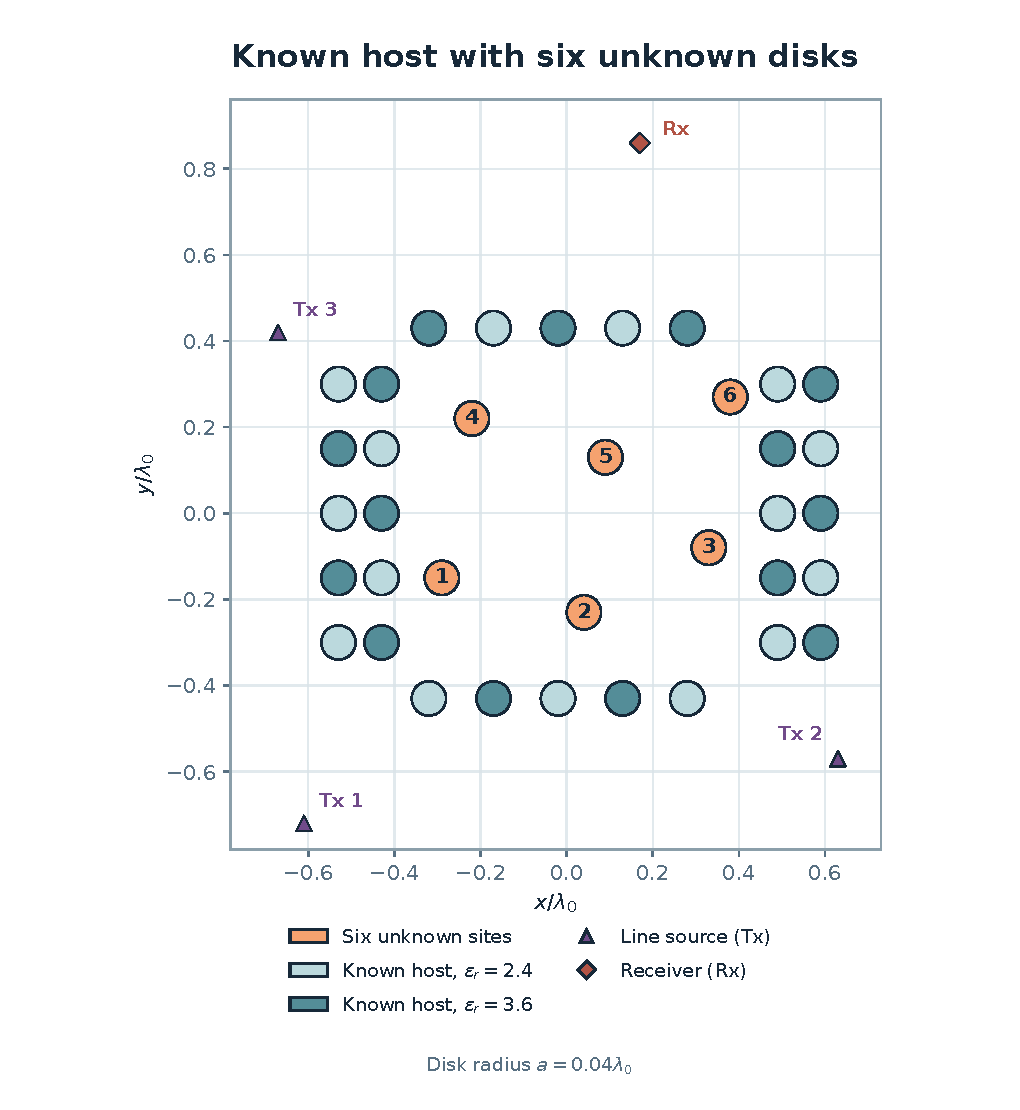
\includegraphics[width=.64\linewidth]{figures/host_geometry.pdf}
\caption{The three illuminations interrogate all six unknowns through the thirty known cells. Removing the known cells at the same material changes the response by $0.07813$ in complex Euclidean norm.}
\end{figure}

With one constant polarization current per disk and testing at its center, write
\[
 J=X(E^{\rm inc}+GJ),\quad y=SJ,\quad X=X_0+P D_zP^T,\quad D_z=\diag(z).
\]
Here $P$ selects six coordinate cells and the other 30 entries of $X$ are known. With $A_0=I-X_0G$, put $U=A_0^{-1}P$, $J_0=A_0^{-1}X_0 E^{\rm inc}$, $H=P^TGU$, $B=P^T(E^{\rm inc}+GJ_0)$, $R=SU$. Elimination gives
\begin{equation}
 F(z)=y_0+R(I-D_zH)^{-1}D_z B,\qquad y_0=SJ_0. \label{forward}
\end{equation}
All repeated scattering between the active and known cells is included.

\section{Outgoing power and the quadratic inverse chart}
For radius $a$, set $\gamma=\pi k_0 a J_1(k_0a)/2$. Off the diagonal, $G_{ij}=i\gamma H_0^{(1)}(k_0|x_i-x_j|)$. Its diagonal is $i\pi k_0a H_1^{(1)}(k_0a)/2-1$. The receiver uses the off-diagonal expression and the incident line source uses $iH_0^{(1)}/4$. These are analytic disk-pulse coefficients. The continuum error of replacing the current by a constant inside each disk is outside the certificate.

\begin{proposition}[Regularity survives host elimination]\label{power}
For distinct equal-radius centers with $\gamma>0$, the Hermitian imaginary part $\imH G=(G-G^*)/(2i)$ is positive definite. Every finite real diagonal loading has a unique forward solution. For any fixed real host and full-rank coordinate selector $P$,
\[
                     \imH H=U^*(\imH G)U\succ0.
\]
\end{proposition}
\begin{proof}
The entries of $\imH G$ are $\gamma J_0(k_0|x_i-x_j|)$, including the diagonal. Its quadratic form divided by $\gamma$ is the angular average of $|\sum_j b_j e^{-ik_0\hat x\cdot x_j}|^2$. Equality would give an outgoing sum of point-source fields with vanishing far field. Rellich's lemma and unique continuation give zero throughout the punctured plane. The distinct logarithmic singularities imply that every $b_j$ vanishes. If $j=XGj$, the entries of $j$ vanish wherever $X_{ii}=0$. On the remaining support $j^*Gj=j^*X^{-1}j$ with the inverse restricted to that support. The right side is real and the imaginary part on the left is positive for nonzero $j$. Finally, with $L=GA_0^{-1}$, multiplication gives $A_0^*(L-L^*)A_0=G-G^*$. Compression by $P$ proves the identity.
\end{proof}
This excludes a real-material pole throughout this model class. A quantitative forward conditioning margin still requires a bound. The ingredients are classical radiation uniqueness and the resolvent congruence.

Let $v=R(I-D_zH)^{-1}$ and $w=v D_z$. Put $t=F-y_0$. For $s$ independent complex illuminations of $2s$ real parameters, $wB=t$ and $v=R+wH$. Choose an invertible row block $B_I$ with complement $J$. With $c=w_J$, $w_I=(t-cB_J)B_I^{-1}$. The affine maps $w(c,t),v(c,t)$ give the real quadratics
\[
                 C_i(c;t)=\operatorname{Im}(w_i\overline{v_i}).
\]
Where all $v_i\ne0$, $C=0$ recovers $z_i=w_i/v_i\in\RR$, subject to the material box. For a chart perturbation $h$, $D^2_cC[h,h]=2\operatorname{Im}((hN)\odot\overline{hNH})$ with $w=w_0+cN$. The Hessian is constant in this chart.

\begin{proposition}[The real Jacobian]\label{jac}
With unscaled $C$, real then imaginary coordinates in each complex block and the above pivot chart,
\begin{equation}
 \det D_cC=(-1)^s \frac{|\det(I-D_zH)|^2}{|\det B_I|^2}\det D_zF. \label{bridge}
\end{equation}
\end{proposition}
\begin{proof}
Off the receiver nodes, $\zeta_i=w_i/v_i$ gives complex coordinates near the real point. Its complex Jacobian in column notation is $D_v^{-1}(I-D_zH^T)$, with real determinant $|\det(I-D_zH)|^2/\prod_i|v_i|^2$. In $\zeta$ coordinates the lower diagonal block for $C$ is $\diag(|v_i|^2)$, since $C_i=|v_i|^2\operatorname{Im}\zeta_i$ at first order, and the upper left block is the physical real $D_zF$. The change $(t,c)\mapsto w$ contributes $(-1)^s/|\det B_I|^2$ with the specified block order. At a real node, $w_i=v_i=0$, the $i$th compatibility row and material derivative column vanish.
\end{proof}
Equation \eqref{bridge} was derived in the earlier six-site study. A pole, a receiver node, an ordinary inverse fold and a degenerate elimination chart require different tests. An isolated physical fold has local algebra $\CC[\xi]/(\xi^2)$ in a regular, non-nodal chart with a unique lift. A multiple complex quotient root alone does not establish a physical fold.
\section{A transition across the entire material box}
The fixed complex observations $y_-,y_+$ are supplied at full precision with the code. Set $\tau=10^{-6}$ (the archived binary value), $y_b=(y_++y_-)/2$, $n=(y_+-y_-)/(2\tau)$ and $y(p)=y_b+pn$. The center $y_c$ of the noisy experiment is the separately recorded forward prediction at the numerical critical material. The rounding difference between $y_b$ and $y_c$ is carried through the calculation. Let
\[
 \mathcal M=\{z\in K:\|F(z)-y_c\|_2\le \rho\},\qquad \rho=5\,2^{-22}.
\]
The entire segment is in the noise ball by convexity and the verified endpoint distances.

\begin{theorem}[Computer-assisted material count]\label{main}
The number of legal materials changes at exactly one level, $p_*$, on the specified observation line. Its position and the counts on either side are
\[
 -2.057\,10^{-18}\le p_*\le -2.056\,10^{-18},\qquad
 \#\{z\in K:F(z)=y(p)\}=
 \begin{cases}2&-\tau\le p<p_*,\\1&p=p_*,\\0&p_*<p\le\tau.\end{cases}
\]
The critical material is an ordinary non-nodal fold with full forward $\sigma_{\min}>0.26124$. Throughout the noisy feasible set the full forward matrix satisfies $\sigma_{\min}(I-XG)>0.25260$.
\end{theorem}

\paragraph{Checking the endpoints independently.}
Complexifying the six real chart quadratics treats $c$ and its formal conjugate $d$ as independent. The equations are linear in $(1,d)$. The 15 maximal minors in $c$ have degree at most four. The leading $15$ by $15$ quartic block is interval-invertible at each endpoint. The 20 monomials of degree at most three therefore span the quotient, so its variety is finite. We isolate 20 distinct $c$ projections by verified contractions and certify full column rank for the lift in $d$ at each projected root. This saturates the upper bound. Conjugate symmetry and uniqueness in the isolation boxes give the real-conjugate lifts. Division to recover a material is checked off the receiver nodes. At $y_-$ there are 16 nonconjugate, two out-of-range and two legal roots. At $y_+$ the counts are 18, two and zero. The six-dimensional Euclidean material separation at $y_-$ is at least $0.561476$.

\begin{center}\small
\begin{tabular}{lrrrrrr}
\toprule & $z_1$ & $z_2$ & $z_3$ & $z_4$ & $z_5$ & $z_6$\\\midrule
Lower slot 6 & 19.12056 & 7.73765 & 4.18712 & 2.58417 & 19.33020 & 25.77097\\
Higher slot 6 & 18.87820 & 7.49460 & 4.35267 & 2.52954 & 19.25972 & 26.17357\\\bottomrule
\end{tabular}
\end{center}

\paragraph{Closing the gap between point counts.}
Parameterize a sheet by $u=z_6-z_6^{\rm ref}$, $z_6^{\rm ref}=25.966536948968322$ as stored, and solve the six real equations for $(z_1,\ldots,z_5,p)$. The bordered Jacobian is $[D_{1:5}F,-n]$. A parametric Krawczyk inclusion proves existence and uniqueness inside each of 55 tubes on $[-0.625,0.625]$. An independently isolated point on each common face belongs to both adjacent tubes. For the resulting $p=g(u)$, implicit differentiation with the full analytic resolvent bounds $-1.306\,10^{-4}\le g''(u)\le-2.42\,10^{-7}$. The endpoint derivatives have opposite signs and both endpoint levels are below $-\tau$. Thus $g$ has exactly one maximum. Its level is bounded from $g(0)$ and $g'(0)$ using the uniform negative curvature. Its tiny offset from zero reflects the deliberate centering of the line.

To establish the count throughout $K$, take the 222 boxes covering $\mathcal M$ from the direct set inversion below. For each box and each overlapping segment of the sheet, hold $z_6$ fixed. Choose a real projection $L:\RR^6\to\RR^5$ with $\ker L=\mathrm{span}(n)$. Enclose $L D_{1:5}F$ on the convex hull between any candidate and the validated point on the sheet at that same $z_6$. For all 1,306 intersections, the enclosure contains only nonsingular matrices. It contains the Jacobian averaged along the material segment. Two distinct points on the measured line at the same $z_6$ would give an average matrix with a nontrivial kernel. The sheet remains inside $K$. Hence the local count is global along this line. Invertibility of the bordered matrix and $g''\ne0$ prove the fold conditions.

For the forward margin on all 222 boxes, factor $A(z)=(I-PD_\delta P^T G A_m^{-1})A_m$ at each cell center $m$. Positive definiteness of $A_m^*A_m-0.2599^2 I$ and $\|\diag(h)P^T G A_m^{-1}\|_F<0.028077$ for the cell half-widths $h$ give the stated result. Verifying this uniform physical bound took 3.36 s.

\begin{figure}[ht]
\centering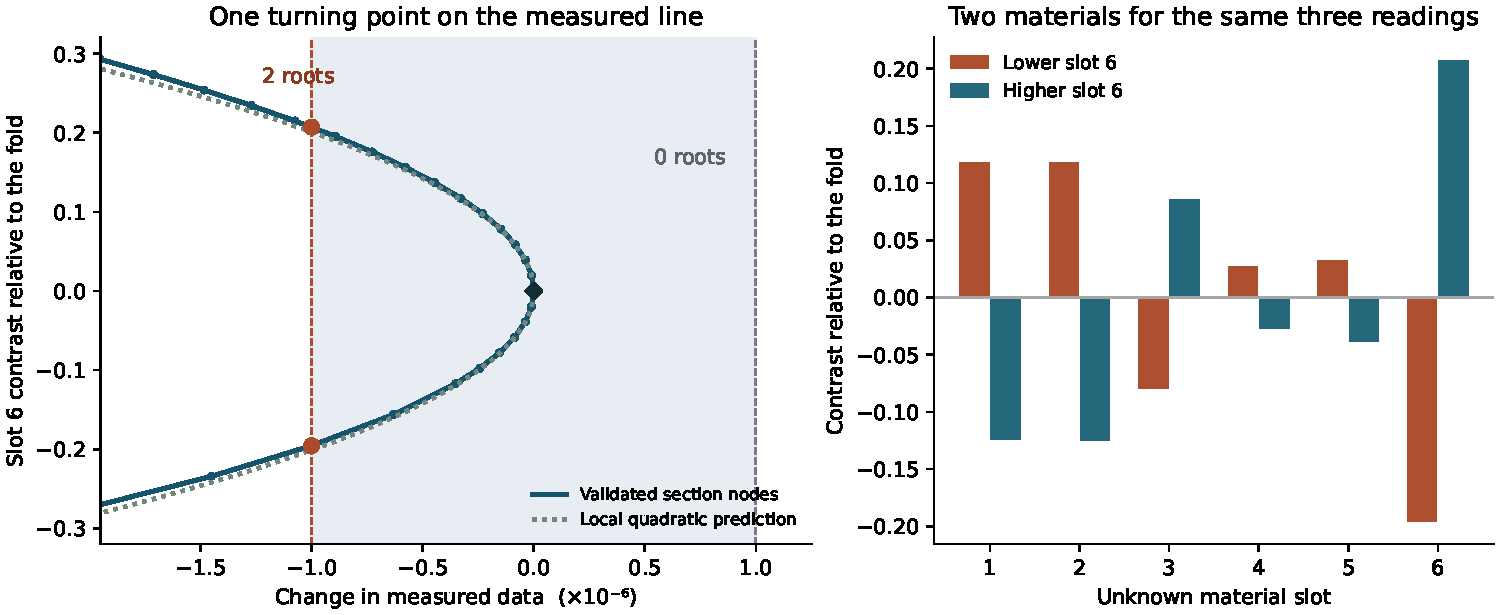
\includegraphics[width=\linewidth]{figures/material_branches.pdf}
\caption{Left, signed data displacement and contrast in the sixth slot on the validated curve. The dotted parabola uses the local fold coefficient. Right, changes of all six materials for the two exact solutions at $y_-$.}
\end{figure}

\paragraph{Which interaction produces the turning?}
The Born map about the calibrated host is $y_0+RD_zB$. Its constant real Jacobian satisfies $\sigma_{\min}>2.2610\,10^{-4}$, so it is injective everywhere. Keeping only the diagonal of dressed $H$ restores full material rank in the verified critical material segment ($\sigma_{\min}>4.9586\,10^{-4}$). In the complete model the minimum receiver factor exceeds $0.00462$ at the fold. At the nearby coordinate-line critical material, unit left and right null directions $\ell,v$ of the measured material Jacobian give $\kappa=\ell^T D^2F[v,v]\simeq-2.54532\,10^{-5}$. The signed displacements along $v$ of the two roots are $-0.27254$ and $0.28894$, compared with the local magnitude $\sqrt{2\tau/|\kappa|}=0.28031$. Along an individual sheet the inverse has square-root dependence in the normal data coordinate. Suppressing inter-slot feedback retains the effect of the host on the incident fields and receiver. This test isolates a cause at the selected materials. Folds elsewhere in the diagonal-only model have not been excluded.

\section{What remains possible after admitting noise}
On a compact material box with regular forward propagation, each connected component of the inverse image of a closed data ball for a square real map contains a central root, a critical material, or a box-boundary point. Indeed, minimize the distance to the center on the component. At an interior regular minimizer of positive distance, the local inverse lifts a radial step towards the center and decreases that distance within the same component. The endpoint $y_+$ gives a concrete corollary: taking it as center leaves zero central roots, but a ball of the same radius $\rho$ still contains the certified critical response. Thus a full central-root catalogue can be empty for a nonempty noisy inverse set. The measured cover below uses the original center $y_c$.

All methods receive the same $K,y_c,\rho$ and analytic model enclosures. Three disjoint positive-volume feasible boxes and two verified paths join the endpoint roots through a neighbourhood of the fold. Each path has eight linear pieces. The full squared residual divided by $\rho^2$ is bounded by 0.70455 along either path. A common noisy datum can therefore be explained by a connected set containing both materials. For any point estimate at that datum, the triangle inequality gives a worst-case error of at least $0.11461$ rms over the six contrasts. The path establishes connectedness between these witnesses. The number of other components of the whole six-dimensional feasible set is undetermined.

For a direct test write $q=\det(I-HD_z)$ and $N=q(F-y_c)$. Each is multiaffine in $z$. The full necessary and sufficient test is $\|N\|^2-\rho^2|q|^2\le0$. The stronger direct SIVIA implementation combines Bernstein enclosures of this polynomial with joint directional bounds on the real residual numerator. In the receiver chart, each set $\mathcal I$ of four columns of $N_0(I-HD_z)$, where $N_0 B=0$, has cofactor weights $\lambda$. With $\alpha$ chosen so that $(I-HD_z)_{:,\mathcal I}\lambda=B\alpha$, feasibility implies
\[
 |(y_c-y_0)\alpha-\sum_{i\in\mathcal I}z_iR_i\lambda_i|^2\le\rho^2\|\alpha\|^2 .
\]
Testing the 15 subsets uses four-variable polynomials and reuses their projections. Each test relaxes the common measurement error. In a verified six-dimensional cube of halfwidth $2^{-23}$, every normalized single-minor score is below 0.734 and the full squared-error score exceeds 1.1676 everywhere. Subdivision alone cannot close this gap for these individual tests.

\begin{center}\small
\begin{tabular}{lrr}
\toprule Global material box, Apple M4 & Direct, joint & Receiver minors\\\midrule
Visits to equal retained fraction $9.984\,10^{-7}$ & 19,102 & 1,874\\
Wall time to this fraction, with test preparation (s) & 0.1237 & 0.0298\\
Including shared upstream physics and certification (s) & 0.2073 & 0.1134\\
Final unresolved boxes at depth 48 & 222 & 345\\
Final retained fraction of original six-volume & $7.887\,10^{-13}$ & $1.226\,10^{-12}$\\
Final wall time including shared upstream work (s) & 0.2214 & 0.1209\\\bottomrule
\end{tabular}
\end{center}
The chart is faster to a matched retained volume here. At a common fine resolution the joint direct method excludes more of the global domain. A small volume alone does not bound error in a specified material coordinate. A mature multihomogeneous \texttt{HomotopyContinuation.jl} run~\cite{bt} tracks 20 paths with zero failures at each endpoint. Warm single-thread runs take 0.0104 s per point before certification, with 21.15 s for the entire Julia process including first compilation and repeated solves. The quotient implementation takes 0.041 and 0.043 s per endpoint including interval leading-rank and root proofs once host enclosures are available. The same certificate accepts the homotopy nominees. A point solver has a different output from an outer cover of all noisy data.
\begin{figure}[ht]
\centering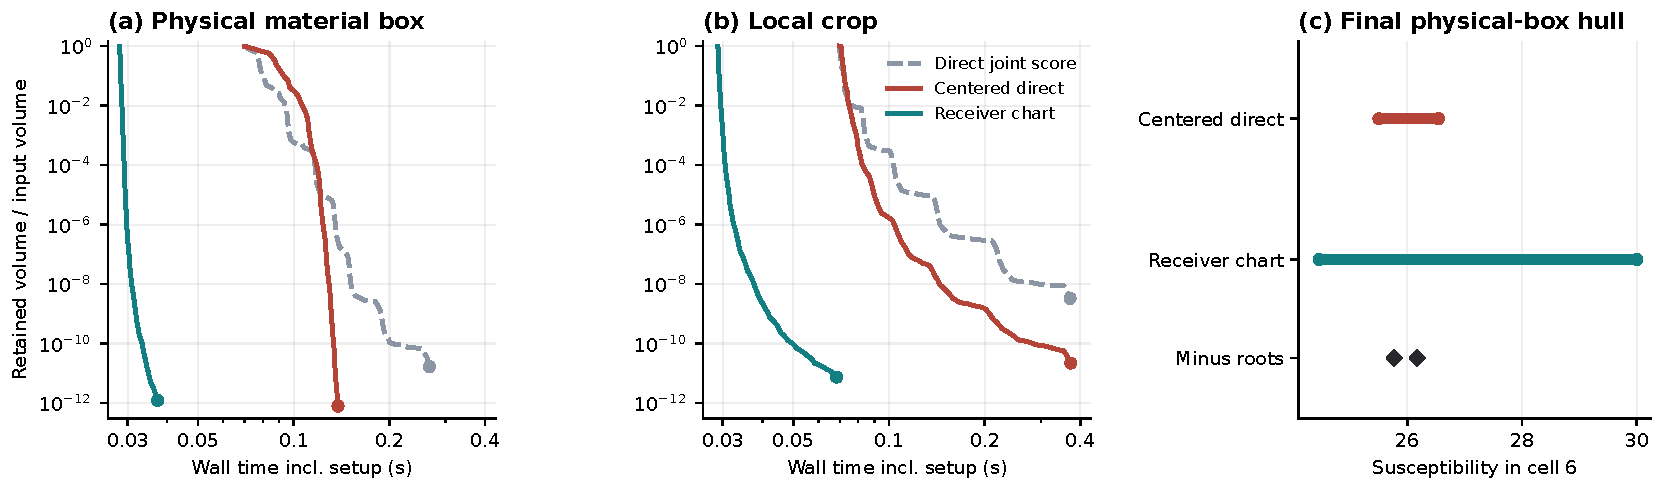
\includegraphics[width=\linewidth]{figures/noisy_cover_frontiers.pdf}
\caption{Matched global and local outer covers on the same noise set. The projection onto the sixth contrast distinguishes the tightness of global results even when both fractions of six-volume are small.}
\end{figure}
\section{Relationship to earlier results and scope}
Everett~\cite{everett96,everett26} and Vasco~\cite{vasco00} established polynomial multi-solution geophysical inversion. Vasco's singular and path-following analyses~\cite{vasco93,vasco94} also concern branching in inverse problems. The transfer representation follows directly from T-matrix completion~\cite{dctmc}. Effective sources and recovery of strength from local fields appear in Foldy--Lax imaging~\cite{chai}. The invisible point-scatterer examples of Kuo and Novikov~\cite{kuo} make the distinction between a node and this non-nodal fold essential. Validated folds~\cite{lessard} and bounded-error set inversion~\cite{sivia} are established techniques.

Two earlier project results concern different experiments (see the \href{https://github.com/migodam/b1-probabilistic-maxwell-imaging/blob/main/research/research_z_alg_r7/THEORY_DERIVATIONS.md}{continuum derivation} and the \href{https://github.com/migodam/b1-probabilistic-maxwell-imaging/blob/main/research/research_z_alg_r14/MATHEMATICAL_THEORY.md}{band-energy proof}). In the homogeneous two-dimensional continuum, the real derivative of finitely many independent outgoing line-source data at a single receiver can be onto through perturbations in an arbitrary open nuisance region. Analytic continuation, Rellich's lemma and the implicit function theorem give local cancellation by small two-sided real material changes there. A separate six-cell example bounds all feedback-controlled choices of three physical ports across a prescribed continuous band by radiated energy. Its quantitative minimax bound uses that geometry, band and noise contract. Neither result supplies a continuum discretization error for the present host.

The contribution here is a complete finite-aperture material-count transition for a specified scattering model with a quantitative physical margin on an entire noisy inverse set. At the two off-critical endpoints, compactness of $K$, isolation of the two interior regular solutions and the positive residual away from those solutions imply persistence of the counts under sufficiently small $C^1$ forward perturbations. The fold itself persists locally under small $C^2$ perturbations. These qualitative openness statements leave the tolerance for fabrication or a continuum forward solver unquantified. The numerical evidence supports a theory and computation paper about material calibration. General imaging speed and reconstruction of unknown support require different evidence.

\paragraph{Reproducibility.}
The \href{https://migodam.github.io/b1-probabilistic-maxwell-imaging/research/z_alg_host_fold/}{study page} provides raw bounds, coordinates, code and a proposition-level literature comparison. Error intervals start with the decimal geometry, analytic Hankel functions and the full host solve, and propagate through the chart, the physical map and both noisy-set tests. Runtime reports identify cached and shared costs.

\begin{thebibliography}{11}\small
\bibitem{everett96} M. E. Everett, Homotopy, polynomial equations, gross boundary data, and small Helmholtz systems, \emph{J. Comput. Phys.} 124 (1996), 431--441. \href{https://doi.org/10.1006/jcph.1996.0070}{DOI}.
\bibitem{vasco93} D. W. Vasco, Degeneracy, singularity and multiple solutions in geophysical inversion, \emph{Geophys. J. Int.} 113 (1993), 434--448. \href{https://doi.org/10.1111/j.1365-246X.1993.tb00898.x}{DOI}.
\bibitem{vasco94} D. W. Vasco, Singularity and branching: a path-following formalism for geophysical inverse problems, \emph{Geophys. J. Int.} 119 (1994), 809--830. \href{https://doi.org/10.1111/j.1365-246X.1994.tb04019.x}{DOI}.
\bibitem{vasco00} D. W. Vasco, An algebraic formulation of geophysical inverse problems, \emph{Geophys. J. Int.} 142 (2000), 970--990. \href{https://doi.org/10.1046/j.1365-246x.2000.00188.x}{DOI}.
\bibitem{everett26} M. E. Everett, Multiple solutions to geophysical inverse problems via tracking flights across a deeply incised model landscape, \emph{Geophys. J. Int.} 247 (2026), ggag432. \href{https://doi.org/10.1093/gji/ggag432}{DOI}.
\bibitem{chai} A. Chai, M. Moscoso and G. Papanicolaou, Imaging strong localized scatterers with sparsity promoting optimization, \emph{SIAM J. Imaging Sci.} 7 (2014), 1358--1387. \href{https://doi.org/10.1137/130943200}{DOI}.
\bibitem{dctmc} H. W. Levinson and V. A. Markel, Solution of the nonlinear inverse scattering problem by T-matrix completion. I. Theory, \emph{Phys. Rev. E} 94 (2016), 043317. \href{https://doi.org/10.1103/PhysRevE.94.043317}{DOI}.
\bibitem{kuo} P.-C. Kuo and R. G. Novikov, Inverse scattering for the multipoint potentials of Bethe--Peierls--Thomas--Fermi type, \emph{Inverse Problems} 41 (2025), 065021. \href{https://doi.org/10.1088/1361-6420/ade282}{DOI}.
\bibitem{lessard} J.-P. Lessard, Rigorous verification of saddle-node bifurcations in ODEs. \href{https://www.math.mcgill.ca/jplessard/Publications_files/saddle_node.pdf}{Author manuscript}.
\bibitem{sivia} L. Jaulin and E. Walter, Set inversion via interval analysis for nonlinear bounded-error estimation, \emph{Automatica} 29 (1993), 1053--1064. \href{https://doi.org/10.1016/0005-1098(93)90106-4}{DOI}.
\bibitem{bt} P. Breiding and S. Timme, HomotopyContinuation.jl: a package for homotopy continuation in Julia, \emph{ICMS} (2018). \href{https://www.juliahomotopycontinuation.org/}{Project and documentation}.
\end{thebibliography}
\end{document}
